\documentclass[10pt,twocolumn]{article}
\usepackage{graphicx}
\usepackage{fancyhdr}
\usepackage{amssymb,amsmath}
\usepackage[usenames,dvipsnames]{color}
\usepackage[colorlinks,citecolor=RedViolet,urlcolor=blue]{hyperref}
\usepackage{doi}
\usepackage{setspace}
\usepackage[paperwidth=8.5in, paperheight=11in,top=1in, bottom=1in, left=1in, right=1in]{geometry}
\usepackage[compact]{titlesec}
\usepackage{abstract}
\usepackage[position=t,singlelinecheck=off,justification=raggedleft]{subcaption}
\usepackage[authoryear,square]{natbib}
\usepackage{aas_macros}
\usepackage{array}
\pagestyle{fancy}
\fancyhead[R]{Veibell \thepage}
\fancyhead[L]{}

\newcolumntype{L}{>{$}l<{$}} %To enable math mode in tables (for saying things like B_z)
\newcolumntype{C}{>{$}c<{$}}
\newcommand{\vinote}[1]{\textcolor{red}{\textbf{#1}}} %If you want \inote{#} instead of just \note #, for inline notes
\def\vnote#1\par{\textcolor{red}{\textbf{#1}}\\} %Make note bold and red, re-add newline
\newcommand{\req}{\ensuremath{\rho_{eq}}}
\newcommand{\inote}[1]{\textcolor{blue}{\textbf{#1}}} %Inline notes in blue
\def\note#1\par{\textcolor{blue}{\textbf{#1}}\\} 

\begin{document}
\title{Relationship between solar wind, $D_{st}$, and plasmasphere trough mass density on one-hour time scales}
\author{
Victoir Veibell\footnote{vveibell@gmu.edu}
\and
R.S. Weigel\footnote{rweigel@gmu.edu}}


\setlength{\parskip}{3ex}
\renewcommand{\labelitemi}{$-$}
\titlespacing{\section}{0pc}{0.2pc}{-1pc}
\titlespacing{\subsection}{0pc}{0.1pc}{-1pc}
\titleformat*{\section}{\normalsize\bfseries}
\titleformat*{\subsection}{\small\bfseries}

\twocolumn[
  \begin{@twocolumnfalse}
\maketitle
\hrule
\begin{abstract}
This paper compares various magnetosphere conditions around the onset of geomagnetic events, defined as decreases in $D_{st}$ below a threshold value or $\rho_{eq}$ above a threshold value. 

\vspace{2em}
\end{abstract}
 \end{@twocolumnfalse}
  ]

\saythanks

\section{Introduction}

The plasma trough is a transition region between the higher density and lower temperature plasmasphere and the lower density and higher energy magnetosphere \citep{Mayr1968ModelMagnetosphereTemperature}.  Inside of the plasmapause, the density is primarily due to ionospheric photoionization; outside of the plasmapause, the density has contributions from the co-rotating plasmasphere and Earthward convecting magnetosphere plasmas.

The dependence of the plasmapause location on geomagnetic activity was observed as early as \cite{Carpenter1966}.  There are well--validated models of the plasmapause boundary, as a function of $L$, $MLT$, and geomagnetic activity (\cite{LemaireEarthsPlasmasphere}, \cite{Moldwin2002ModelPlasmapause}, \cite{OBrien2003EmpiricalPlasmapause}).  Models also exist for the plasmasphere density (\cite{Gallagher1988EmpiricalModelPlasmasphere}; \cite{LemaireEarthsPlasmasphere}).

The dependence of the plasma trough density on geomagnetic and solar wind conditions has not been extensively studied until the past decade (\cite{Takahashi2006}; \cite{Takahashi2010}; \cite{Denton2016}). Earlier works that considered profiles of electron number density found a significant dependence on the plasmasphere boundary on geomagnetic activity, but there the relationship between geomagnetic activty and density in the plasma trough (\cite{Chappell1970}; \cite{Anderson1993}) was not explicitly considered.

\cite{Lotoaniu1999PlasmaMassDensity} used measurements from the Plasma Wave Experiment instrument on the CRRES satellite and compared in-situ measured plasma mass density to that inferred by ground-based ULF wave measurements from the CANOPUS array. By extending the ground footprints to the plasmatrough, they found agreement between the two methods for certain plasmapause conditions.  \vinote{More details}

\cite{Takahashi2006} estimated magnetospheric mass density using measurements from the CRRES satellite during a 73-day period in 1991 (observations were made when CRRESS was in an elliptical, near equatorial orbit and primarily in the plasma trough region). They found that the average ion mass, $M=\rho/n_e$, had some correlation with geomagnetic activity, with more negative hourly $D_{st}$ values corresponding to higher $M$ and 1.5- and 3-day averages of $K_p$ corresponding to higher $M$ (3-hour averages of $K_p$ had little visual correlation with $M$). The mass density estimates were obtained from CRRES observations in the MLT range of 12:00 and 18:00 with most observations having L between 5 and 7 $R_E$.

\cite{Denton2006} found a weak relationship between $D_{st}$ and and $K_p$ and the field line distribution of $\rho$ using observations of the first three toroidal Alfv\'en harmonic frequencies for $L$ in the range of 6-8$R_E$.  A more pronounced peak in the distribution along a filed line near the equator was found for lower $D_{st}$ and larger $K_p$.  The equatorial value of $\rho$ appeared identical for the bins of $D_{st}$ (-142 to -31 nT and -31 to 37 nT) and $K_p$ (1.5 to 3.4 and 3.4 to 5.9) considered .

\cite{Takahashi2010} developed a mass density dataset using measurements from the Space Environment Monitor instruments on the Geostationary Operational Environmental Satellites (GOES) satellites from 1980 through 1992, with most measurements in the range of $L=6.8\pm0.2 R_E$. The mass density $\rho$ was estimated using the the Alfv\'en wave velocity relationship, $V_A=B/\sqrt{\mu_0\rho}$ a magnetic field model, and a numerical solution to a wave equation with an ionospheric boundary and the assumption of a zero resistance ionosphere.  The equatorial mass density, $\rho_{eq}$, was derived from the estimated mass density using a power law dependence on the geocentric distance to the field line of the observation, $R$, $\rho=\rho_{eq}L/(R/R_E)$.  They found a high correlation ($\sim 0.93$) between 27-day averages of F10.7 and 27-day medians of $\rho_{eq}$.

\cite{Takahashi2010} noted that downward spikes in the $D_{st}$ index coincided with with significant changes in $\rho_{eq}$ for $L$ near 6.8~$R_E$. For five storms, two had $\rho_{eq}$ spikes after the $D_{st}$ drop, two had $\rho_{eq}$ spikes before the drop, and one showed little change in $\rho_{eq}$.  A key result was that when daily-averaged measurements were considered, an enhancement in $\rho_{eq}$ appeared on the same day as minimum $D_{st}$.

\cite{Yao2008} studied the relationship between $D_{st}$ and the number density of low-energy $O^+$ in different regions (ring current and plasma sheet) using the TEAMS and ESA instruments on the low-altitude and high-inclination orbiting FAST satellite and found that the average $N_{O^+}$ across the sampled L-shells (2-14) had a strong correlation (0.88) \inote{With what?}.  Although the correlation in the plasma trough was not calculated, the data presented \inote{for X events} show that the variations in $N_{O^+}$ tended to appear near $D_{st}$ minimum ($\pm$ 2~hours).

\cite{Denton2016} ...

The results in the papers discussed indicate that (1) the mass density in the plasma trough region is best correlated with $F10.7$ and (2) there exists a much weaker relationship between mass density and the geomagnetic activity indices $K_p$ and $D_{st}$.  In this work we consider the dependence of mass density estimates in the \cite{Takahashi2010} and attempt to identify and statistically characterize the relationship between geomagnetic activity with mass density in the plasma trough region.  In addition, we attempt to identify solar wind processes that may drive changes in mass density. 

There are several issues that are addressed in detail: (1) the plasma density measurements are sparse, (2) The plasma trough density has a high correlation with F10.7, and geomagnetic and solar wind parameters also correlate with F10.7, (3) the dependence of mass density on the north/south component of the solar wind magnetic field is expected to be nonlinear. For northward IMF, corresponding to low solar wind driving of the magnetosphere, the plasmasphere can expand past geosynchronous orbit where trough estimates of mass density are made resulting in an increase in observed density that are not due to solar wind driving; for southward IMF, events studies have shown an increase in mass density associated with strong southward IMF and enhanced magnetospheric activity (\cite{Takahashi2010}; \cite{Yao2008}).

Issue (1) is addressed by considering in detail the number of observations that are used in epoch averages around the time of two types of events, decreases in $D_{st}$ below a threshold, and increases in $\rho_{eq}$ above a threshold.  Issue (2) is addressed using various methods to remove or isolate the F10.7 dependences.  Issue (3) is addressed by considering epochs and linear correlations independent of the direction of the IMF along with separation of the epoch averages based on the northward and southward IMF.

In addition, we consider the influence of time averaging by comparing results using daily means and medians and hourly means and medians of solar wind and magnetospheric parameters.


\section{Data Preparation and Overview}

The parameters $\rho_{eq}$ and $F_{10.7}$ used in this work are from the dataset of \cite{Denton}, which was used in \cite{Takahashi2010}; data are available from 1980 through 1991 from GOES 2,3,5, 6 and 7.  All other parameters used are from \cite{Kondrashov2014ReconstructionOfGaps} from 1972 through 2013, which are on a 1--hour time grid. $\rho_{eq}$ is the inferred equatorial mass density based on the 3rd harmonic torodial frequency of magnetic field measurements as described in \cite{Takahashi2010}.  The smallest cadence for $\rho_{eq}$ values is 10 minutes.  To compute an hourly median over the same interval for which the solar wind parameters were averaged, the median of all $\rho_{eq}$ values in a given hour window was used.  Fill (NaN) values were used for hours in which no measurements were available.  In cases where $\rho_{eq}$ was available from multiple GOES satellites at the same time, the value from GOES 6 was selected.  In the dataset, measurements from GOES 6 had the longest time span of coverage.  An overview of the data used is shown in Figure~\ref{AllData}.

In this work, events are defined to occur when $D_{st}$ or $\rho_{eq}$ crosses a threshold value, as indicated by horizontal dashed lines in their respective panels of Figure~\ref{AllData}.

Figure~\ref{ccplot} shows the long-term trends of $log(\rho_{eq})$ from GOES 6 and $F_{10.7}$ computed using the median values in 27-day non-overlapping windows.  A scatter plot of these two lines is shown in the lower panel of Figure~\ref{ccplot}.  The linear correlation for GOES 6 using all measurements is found to be $0.94$, which is the same value documented by \cite{Takahashi2010} who used measurements from all satellites in the time interval of 1980 through 1991 using the constraint $0600 \leq MLT \le 1200$, $K_{p3d}\ge1.0$ and $D_{st}\ge -50$~nT.  Our 27-day correlations for GOES 2, 5, and 7 are 0.81, 0.78, and 0.87, and the time range of coverage of measurements from these satellites are 1980-01-01/1983-05-16, 1983-01-01/1987-02-28, and 1983-05-27/1991-08-29 respectively.

\section{Epoch Average Results}

Two types of events are considered. The first is a drop in the $D_{st}$ index \vinote{Cite Kyoto} below the threshold of -50~nT. These types of events are considered in order to determine if there is a well-defined $\rho_{eq}$ dependence on geomagnetic activity/storms as indicated by $D_{st}$ index.  It is expected that the plasmasphere will exhibit two responses near these threshold crossings.  First is the movement of the plasmasphere earthward (\cite{LemaireEarthsPlasmasphere}) and the second is a possible change in density due to magnetospheric processes. 

The second type of event is an increase in $\rho_{eq}$ above a threshold of 20~amu/cm$^3$.  It is expected that these increases will typically occur after period of quiet geomagnetic activity. In this case, the plasmapause boundary may move outward past geosynchronous orbit and the increase will be due to measurements being made inside the plasmapause.  A second possible reason for the increase could be due to magnetospheric processes.

\subsection{$D_{st}$ Events}

Our first analysis uses data only from the time interval 1989-1991, which corresponds with the interval used in the analysis in \cite{Takahashi2010}. In this interval, there were 329 $D_{st}$ events and 70 $\rho_{eq}$ events.  For both types of events, the hour of the threshold crossing defines the zero epoch time, and for each event, $4\cdot24$ hours were considered before each event and $8\cdot24$ hours after each event.  To compute the epoch averages on a daily time scale, the median value of all available measurements for all events centered on a window of $\pm 12$ hours of the epoch zero hour was computed, and these averaging windows were shifted in increments of $24$~hours. Similar results are obtained if we first reduce each event time series to have a 1-day cadence by computing medians in 1-day bins and then compute the medians across events.  Error bars for each parameter are the standard deviation of the values used in computing the median divided by the square root of the number of values used.

The stack plot in the upper panel of Figure \ref{DailyAveragedDstEvents} shows the epoch averages for these events.  The minimum $D_{st}$ median is $-48$~nT.  Consistent with \cite{Takahashi2010}, $D_{st}$ events correspond to elevated $\rho_{eq}$, although the magnitude of increase observed here is $1.5$ amu/cm$^3$ (from 18 to 19.5~amu/cm$^3$) instead of the increase of $\sim 10$ amu/cm$^3$ found in Figure 11 of \cite{Takahashi2010}.  The vertical green bars in the $\rho_{eq}$ plot show the number of $\rho_{eq}$ values that were used to compute the medians and error bars.  For the non-\req\ medians, the number of measurements used in computing the medians is typically equal to the number of events, which is much larger than the number of \req\ values as we used all available measurements instead of restricting to only values where a non--fill $\rho_{eq}$ value existed.

In the lower panel of Figure \ref{DailyAveragedDstEvents} it is shown that the trends seen in the analysis of 1989-1991 also hold for the entire span of measurements from GOES 6, which spans 1983-1991 - a small elevation on the day of the event relative to the day before and day after, with median averages after the day of the event being slightly lower than that before.  

To determine if the magnitude of the density medians on a given day were statistically different than another day, we used a two-population t-test.  For the interval of 1989-1991, corresponding to the top panel of \ref{DailyAveragedDstEvents}, the null hypothesis that any of the medians from days -1, 0, and 1 are different from each other is rejected with a maximimum p value of \vnote{??}.

   Days     p
-1 and 0
-1 and 1
 0 and 1

Caption: Results of test on different between means of $\rho_{eq}$ shown in the top panel of \ref{DailyAverage} on days near or on the day of a $D_{st}$ event.  A difference in the means can be rejected with a probability of false rejection of $p$.

   Days     p
-1 and 0
-1 and 1
 0 and 1

Caption: Results of test on different between means of $\rho_{eq}$ shown in the bottom panel of \ref{DailyAverage} on days near or on the day of a $D_{st}$ event.  

Both of the results in \ref{DailyAveragedDstEvents} indicate that there is not a statictically significant change in medians of $\rho_{eq}$ on the day before and day after a threshold crossing in $D_{st}$.  

Because the dynamics of the magnetopshere take place on a time scale of less than one day, we have also considered hourly averages as shown in the top panel of \ref{HourlyAveragedDstEvents}.  A total of 668 events were found in the interval of May 1983 through August 1991 with an average duration of 9 hours and a median duration of 3 hours.  The error bars were computed in the same way as \ref{DailyAveragedDstEvents}.  In this plot, the overall trend is similar to that found in the bottom panel of \ref{HourlyAveragedDstEvents} - $\rho_{eq}$ is slighly elevated at the time of the threhshold crossing of $D_{st}$ with respect to the values one day before and after, but the elevation is small and in general not statistically significant.  At this timescale no obvious change in mass density at hourly timescale is visible. This points to an issue with only looking at long-timescale trends between density and $D_{st}$, and allows for the possibility that other factors are influencing the long term correlation because there is no obvious connection on a short timescale.  One possibility is that, as suggested in \cite{Takahashi2010}, $F_{10.7}$ plays a significant role in driving long term density values which biases the long-term correlation of density and $D_{st}$.

Results of test on different between means of $\rho_{eq}$ shown in the bottom panel of \ref{DailyAverage} on days near or on the day of a $D_{st}$ event.  

It was found that $\rho_{eq}$ enhancements do not clearly correspond to a signature in $D_{st}$, but that there is a trend for such enhancements to occur when $B_{z}$ in the IMF is positive.  This is consistent with \cite{Takahashi2010} who note that very large increases in $\rho_{eq}$ often corresponded to movement of the plasmasphere to beyond geosynchronous distances. 

This method finds 669 periods of $D_{st}$ crossing beneath the selected threshold between May 1983 and August 1991 with an average duration of 9 hours and a median duration of 3 hours \vinote{Make sure I defined "duration"}. Figure \ref{HourlyAveragedDstEvents} shows the average values of all events over a window of 24 hours before onset and 48 hours after. Figure \ref{HourlyAveragedDstEvents}a shows events selected by looking for event onsets where $D_{st}$ crossed a threshold of $-40$~nT. The dashed red lines indicate plus and minus one standard deviation of values from all events that were used to compute the median. The final plot in the stack shows both $\rho_{eq}$ and a bar plot of how many valid data points went into the $\rho_{eq}$ average. Since $\rho_{eq}$ comes from a sparser dataset, it has less valid points contributing to the averages than the other parameters in the stack. 

Figure \ref{HourlyAveragedDstEvents} shows a definite spike in the $Z$ component of the magnetic field, as well as the defined drop in $D_{st}$, but no obvious change in mass density at an hourly timescale. This points to an issue with only looking at long-timescale trends between density and $D_{st}$, and allows for the possibility that other factors are influencing the long term correlation since there's no obvious connection on a short timescale. One possibility is that, as suggested in \cite{Takahashi2010}, $F_{10.7}$ plays a significant role in driving long term density values which biases the long term correlation of density and $D_{st}$.

The bottom panel of \ref{HourlyAveragedDstEvents} contains the events shown in the top panel under the constraint that $D_{st}$ remained below -50~nT for at least twelve hours after the event onset time.

\subsection{$\rho_{eq}$ Events}

An alterntive type of event can be defined that corresponds to large increases in $\rho\ $.  In finding $\rho_{eq}$ events, all fill values were replaced with linearly interpolated values. \vinote{Not including \req\ events?}

Figure~\ref{HourlyAveragedRhoEvents} shows the epoch time series for events in which an increase of $\req\ $ above $20$~amu/cm$^2$ defines the start of the event.  Here we see the expected result that such events tend to be associated with positive $B_z^{IMF}$.  To determine if the sign of $B_z^{IMF}$ influences the $\rho\ $ epoch time series, we separated the events by the average of $B_z^{IMF}$ in a time window of $4$~hours.  

Figure~\label{fig:RhoBinned}(a) shows the 
The epoch curves for $B_z^{IMF}\geq=0$ (257) events and $B_z^{IMF}\ge=0$ (139) have no statistically signifiant difference.

\section{F10.7 dependence}
In an effort to analyze the dependence of $\rho_{eq}$ on $F_{10.7}$, a few tests were performed. \cite{Takahashi2010} mention a strong correlation between the two. The long term correlation could be a bias for $D_{st}$'s effects, so a linear model was created, recreating mass density purely from $F_{10.7}$ in the form of $\rho_{eq}(t)=a\cdot F_{10.7}(t)$. This re-created $\rho_{eq}$ shows around a 45\% correlation with the actual $\rho_{eq}$, suggesting a strong influence, while doing the same procedure with $D_{st}$ shows only a 20-25\% correlation. 

Figure \ref{f107bin} takes the events and bins them by the value of $F_{10.7}$ at event onset, then looks at both $\rho_{eq}$ and $B_z$. Error bars calculated in the same manner as before are added to the highest and lowest bins. A significant difference is seen in $\rho_{eq}$ between events taking place during periods of high $F_{10.7}$ and low $F_{10.7}$, while a much less significant, but still noticeable, difference is seen in $B_z$. Also of interest is how $\rho_{eq}$ only sharply reacts to $D_{st}$ events during periods of high $F_{10.7}$. The positive relationship seen in \cite{Takahashi2010} could be due to the short time period looked at, and that it coincides with periods of higher $F_{10.7}$.

Looking at GOES 2,5,6, and 7 shows that this post-onset $D_{st}$ spike happens in almost every case for periods of high $F_{10.7}$. Creating a linear model directly relating variables (and combinations of variables) to $\rho_{eq}$ also shows that $F_{10.7}$ most often has the highest correlation with $\rho_{eq}$. A sample of these correlations is shown in Table \ref{perltable}. The correlations were made by training a one-input linear model of 5-hour post-onset medians of each variable (or variables) against the median of $\rho_{eq}$ at, and four hours after, event onset. This was done by randomly sampling half of the data, generating the model, and testing against the other half, doing this process 100 times and then taking the median correlations.

\newpage
\footnotesize
\bibliographystyle{plainnat}
\bibliography{paper}

\clearpage
\section{Figures}

\begin{figure}[htp!]
\centering
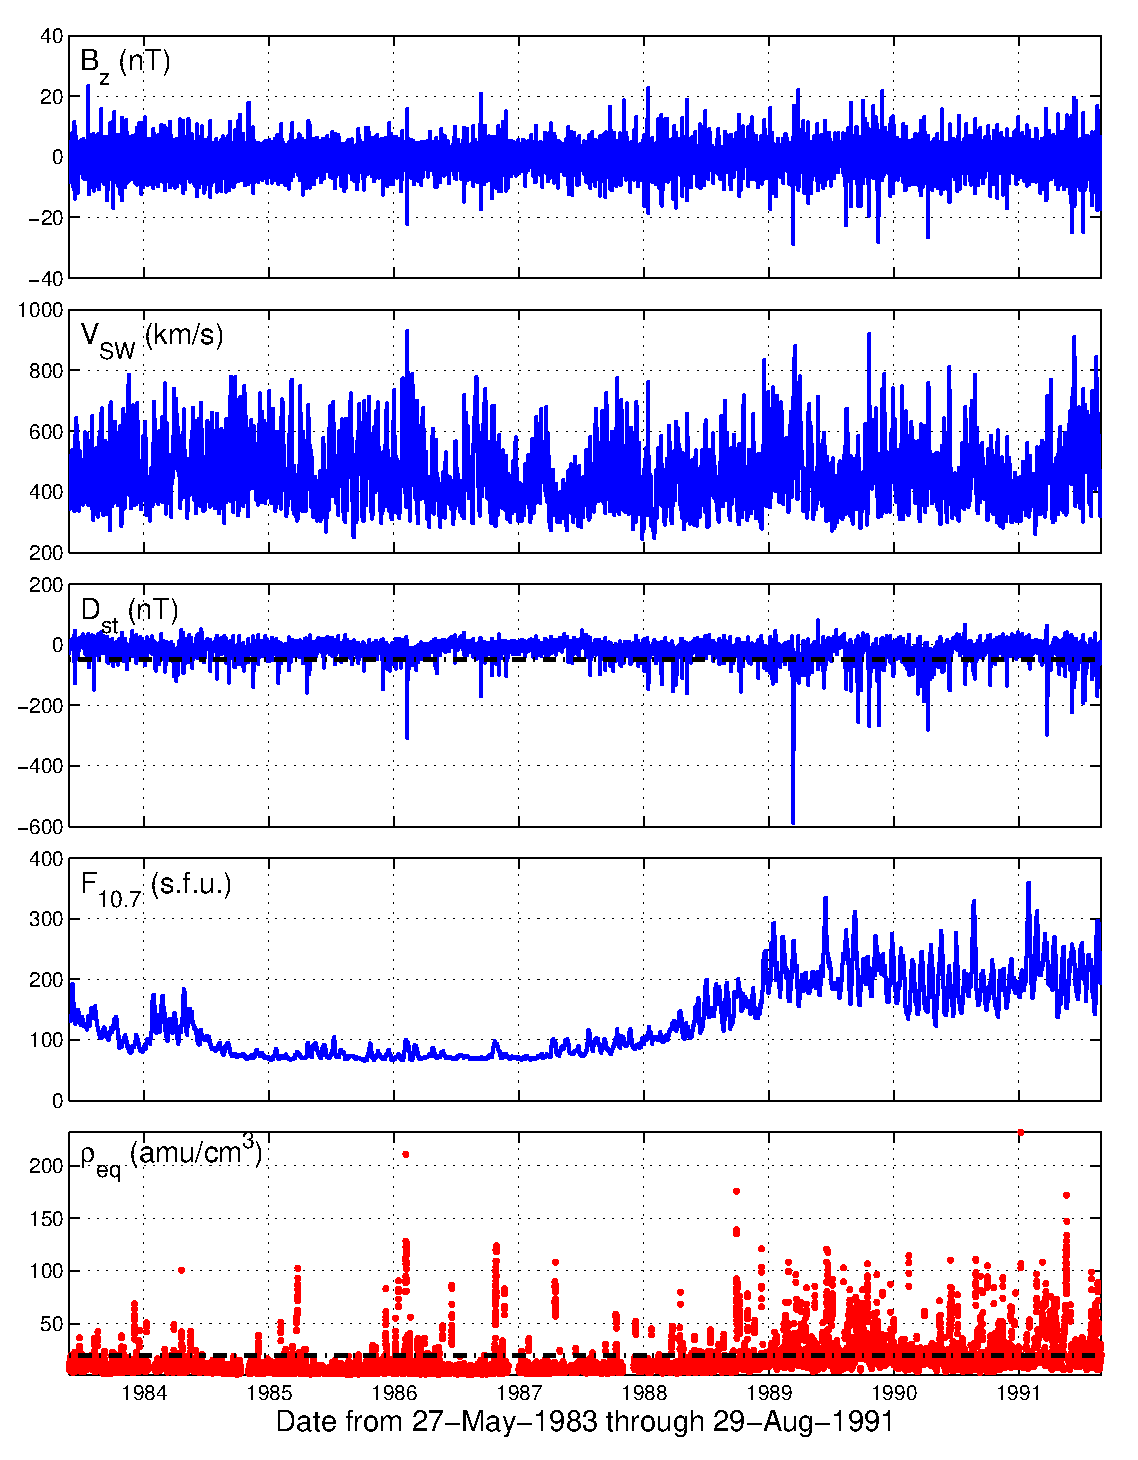
\includegraphics[scale=0.45]{figures/alldata-GOES6-1983-1991.eps}
\caption{Overview of data used in this article. The top four panels show parameters from \cite{Kondrashov2014ReconstructionOfGaps} and the bottom panel contains $\rho_{eq}$ based on GOES 6 measurements from \cite{Denton} after interpolation and averaging described in the text. Dashed horizontal lines in the $D_{st}$ and $\rho_{eq}$ panels indicate sample event cutoff thresholds of $D_{st} = -50$~nT and $\rho_{eq} = 20$~amu/cm$^3$} considered in Section~3.
\label{AllData}
\end{figure}

\begin{figure}[htp!]
\centering
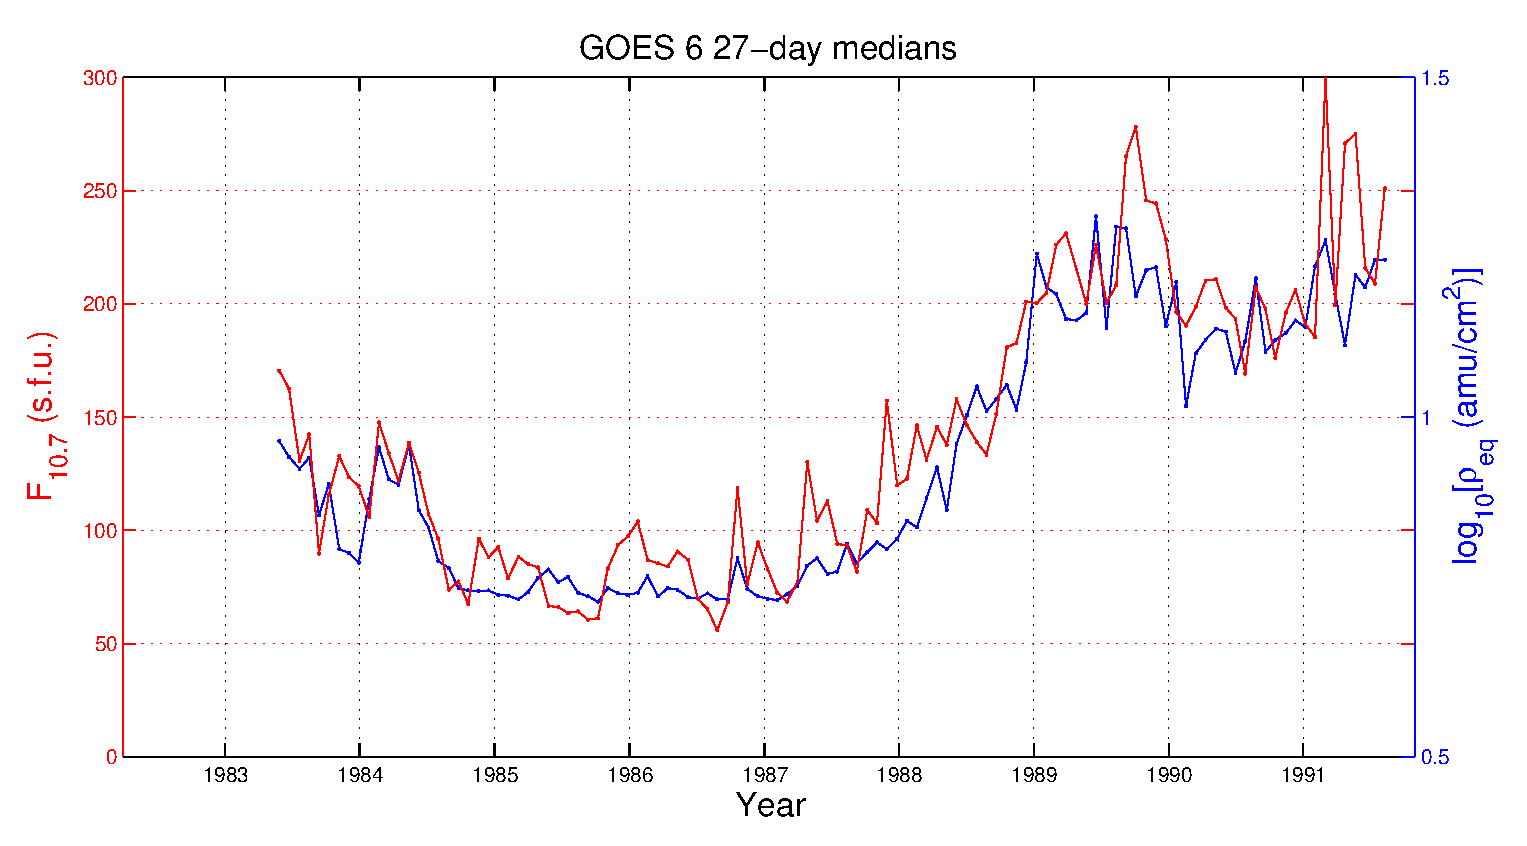
\includegraphics[scale=0.40]{figures/F107MD27d-GOES6.eps}
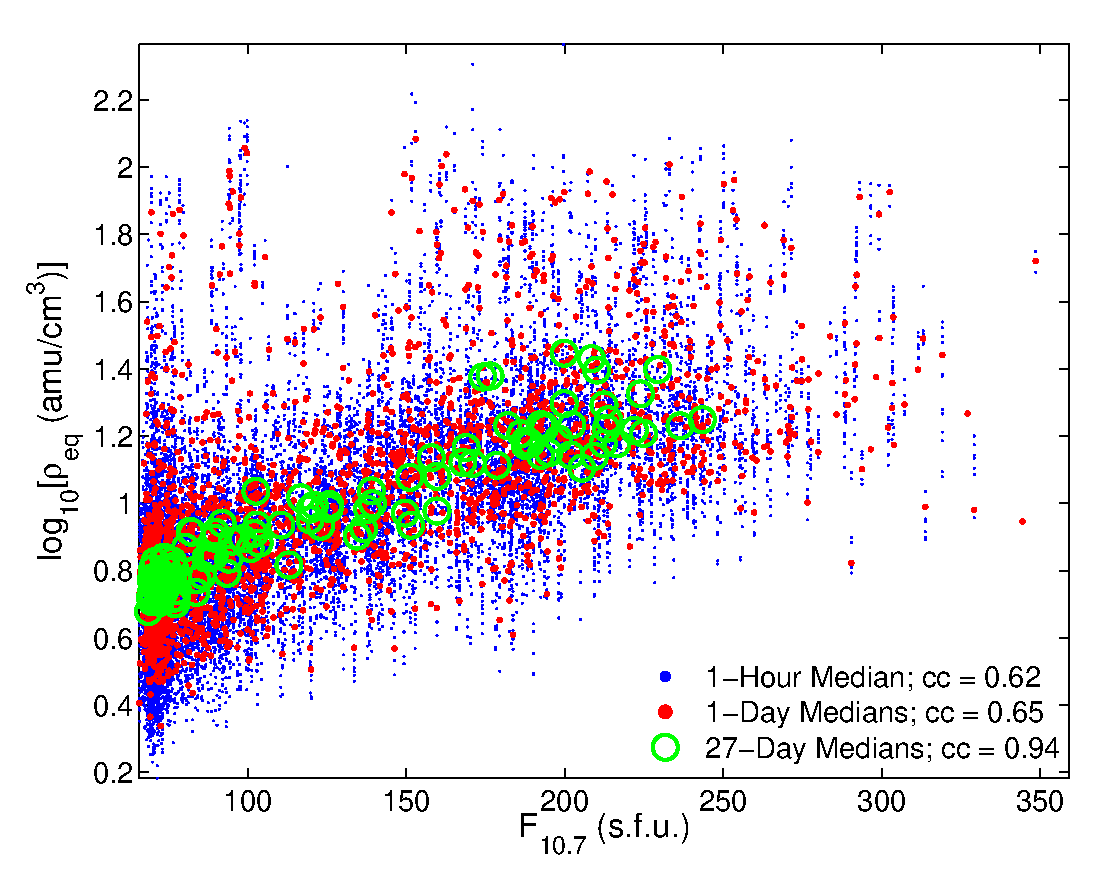
\includegraphics[scale=0.40]{figures/ccplot-GOES6.eps}
\caption{Top: 27-day non-overlapping medians of $F_{10.7}$ and $\log(\rho_{eq})$ from GOES 6. Bottom: Correlation between $\log(\rho_{eq})$ and $F_{10.7}$ using medians in non-overlapping hour, day, and 27-day windows.}
\label{ccplot}
\end{figure}
\clearpage

\begin{figure}[tp!]
\centering
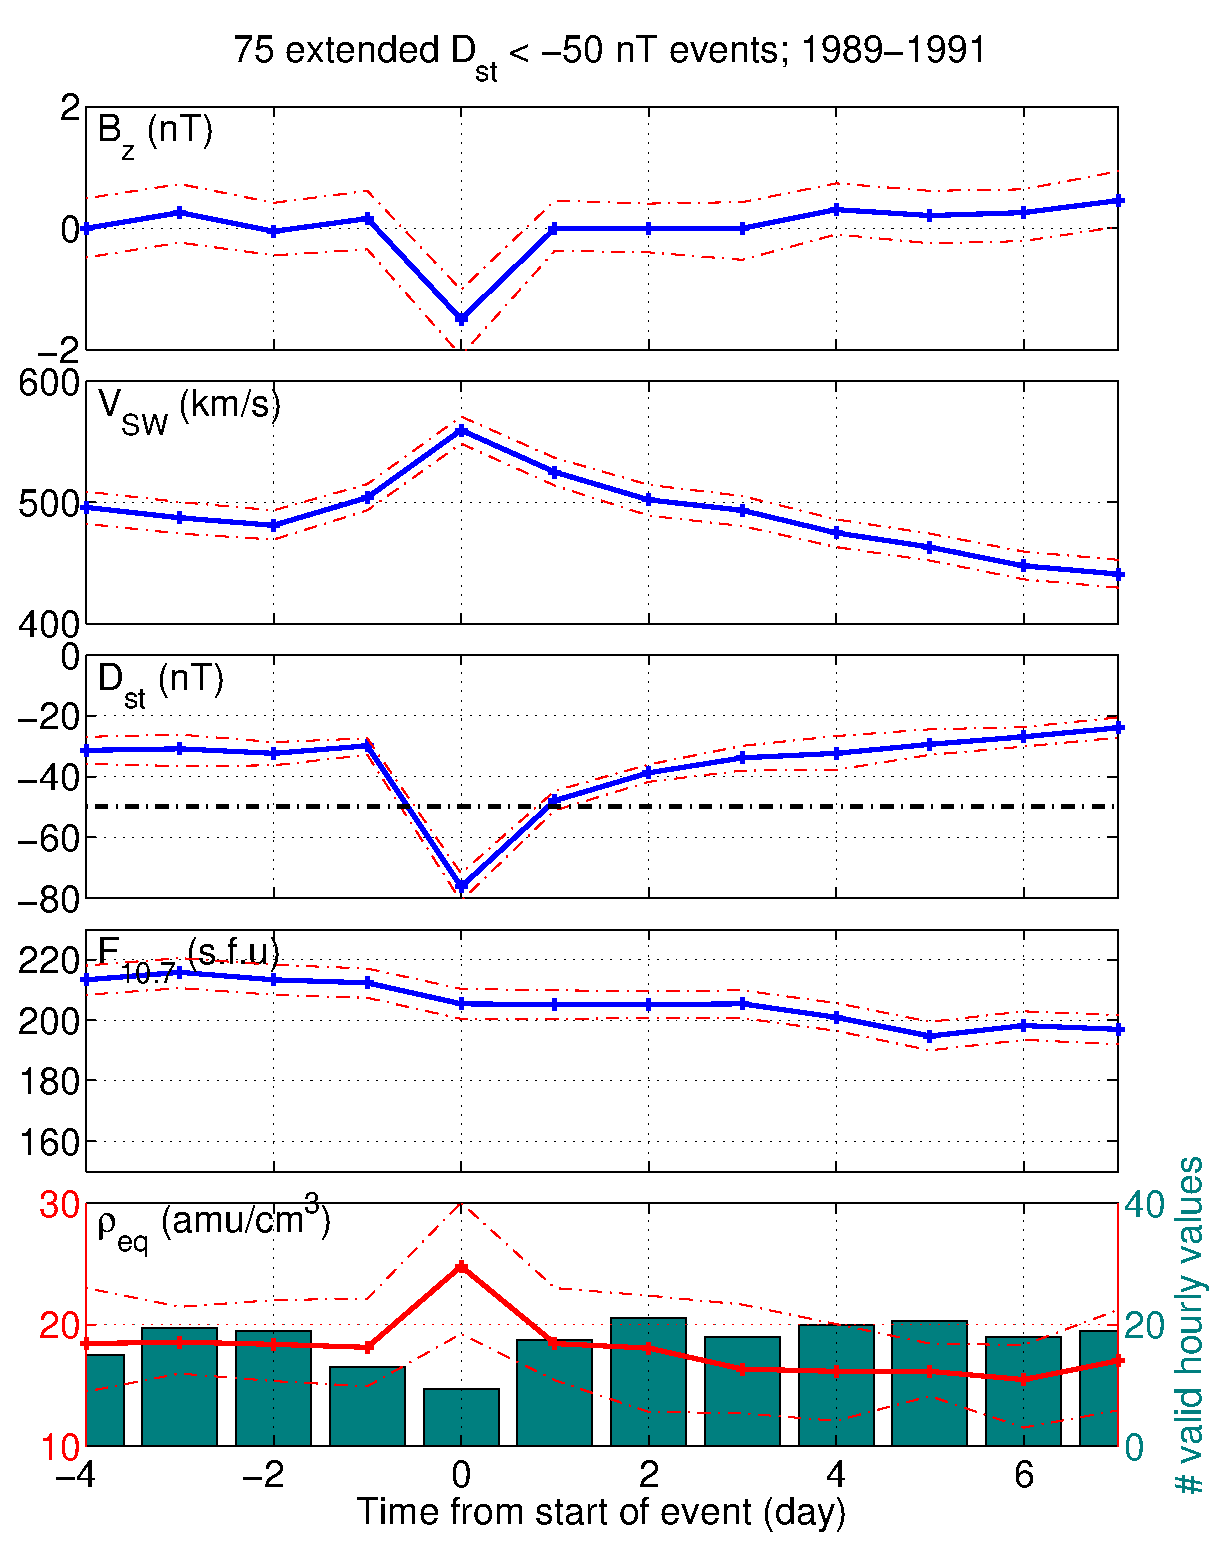
\includegraphics[scale=0.40]{figures/stormavs-dst-50-tak-GOES6.eps}
\rule[1ex]{5cm}{1pt}
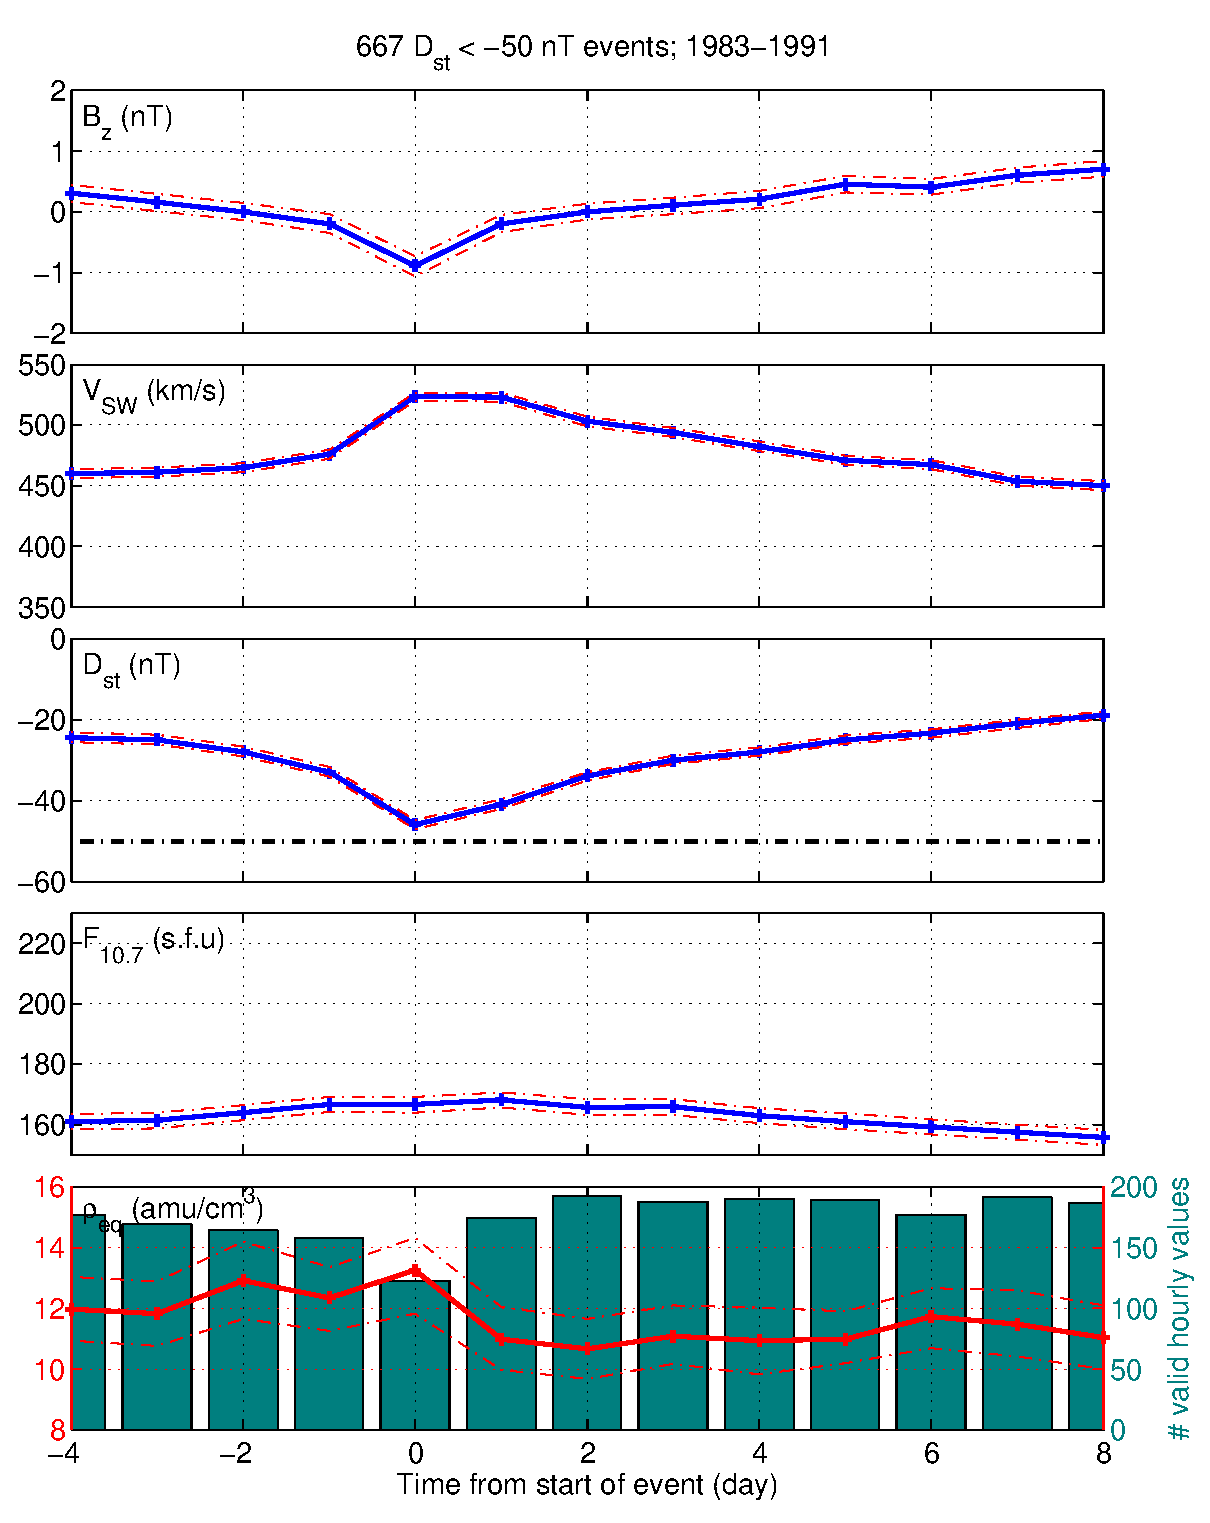
\includegraphics[scale=0.40]{figures/stormavs-dst-day-GOES6.eps}
\caption{$D_{st}$ events from GOES 6 using daily medians. Top: Events in the interval 1989-1991; compare to \cite{Takahashi2010} Fig.~11. Bottom: Events in the interval 1983-1991.}
\label{DailyAveragedDstEvents}
\end{figure}

\begin{figure}[tp!]
\centering
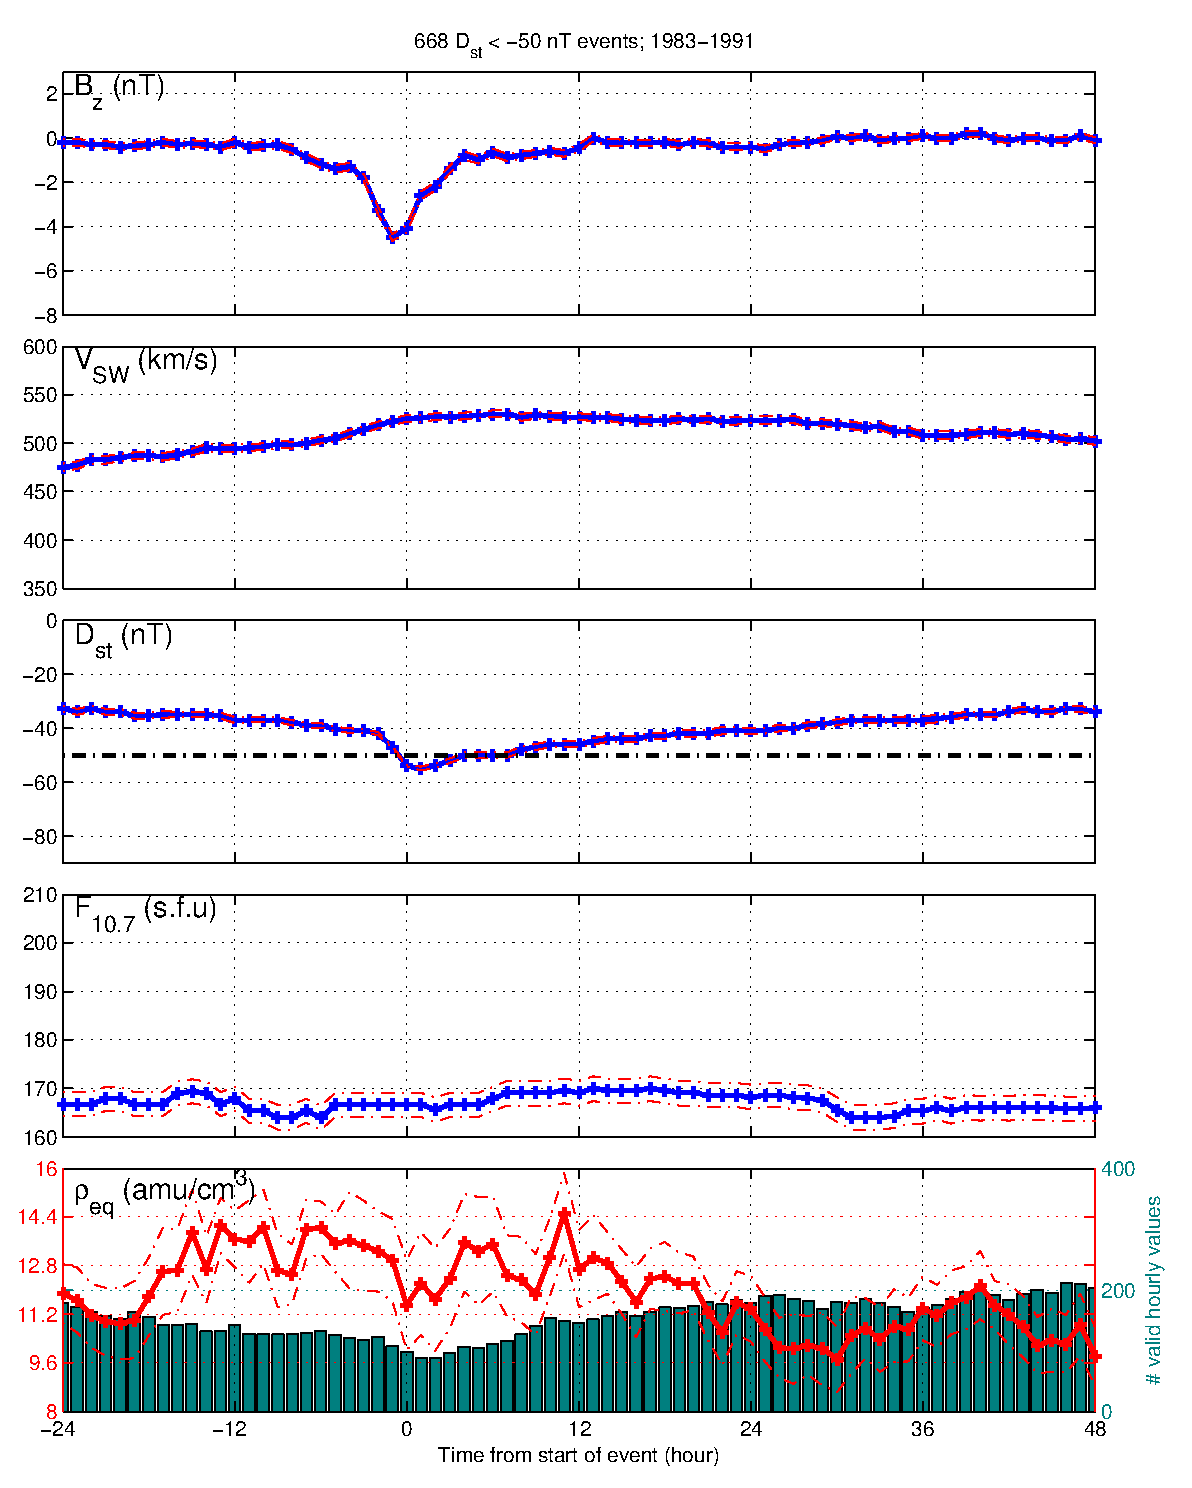
\includegraphics[scale=0.40]{figures/stormavs-dst.eps}
\rule[1ex]{5cm}{1pt}
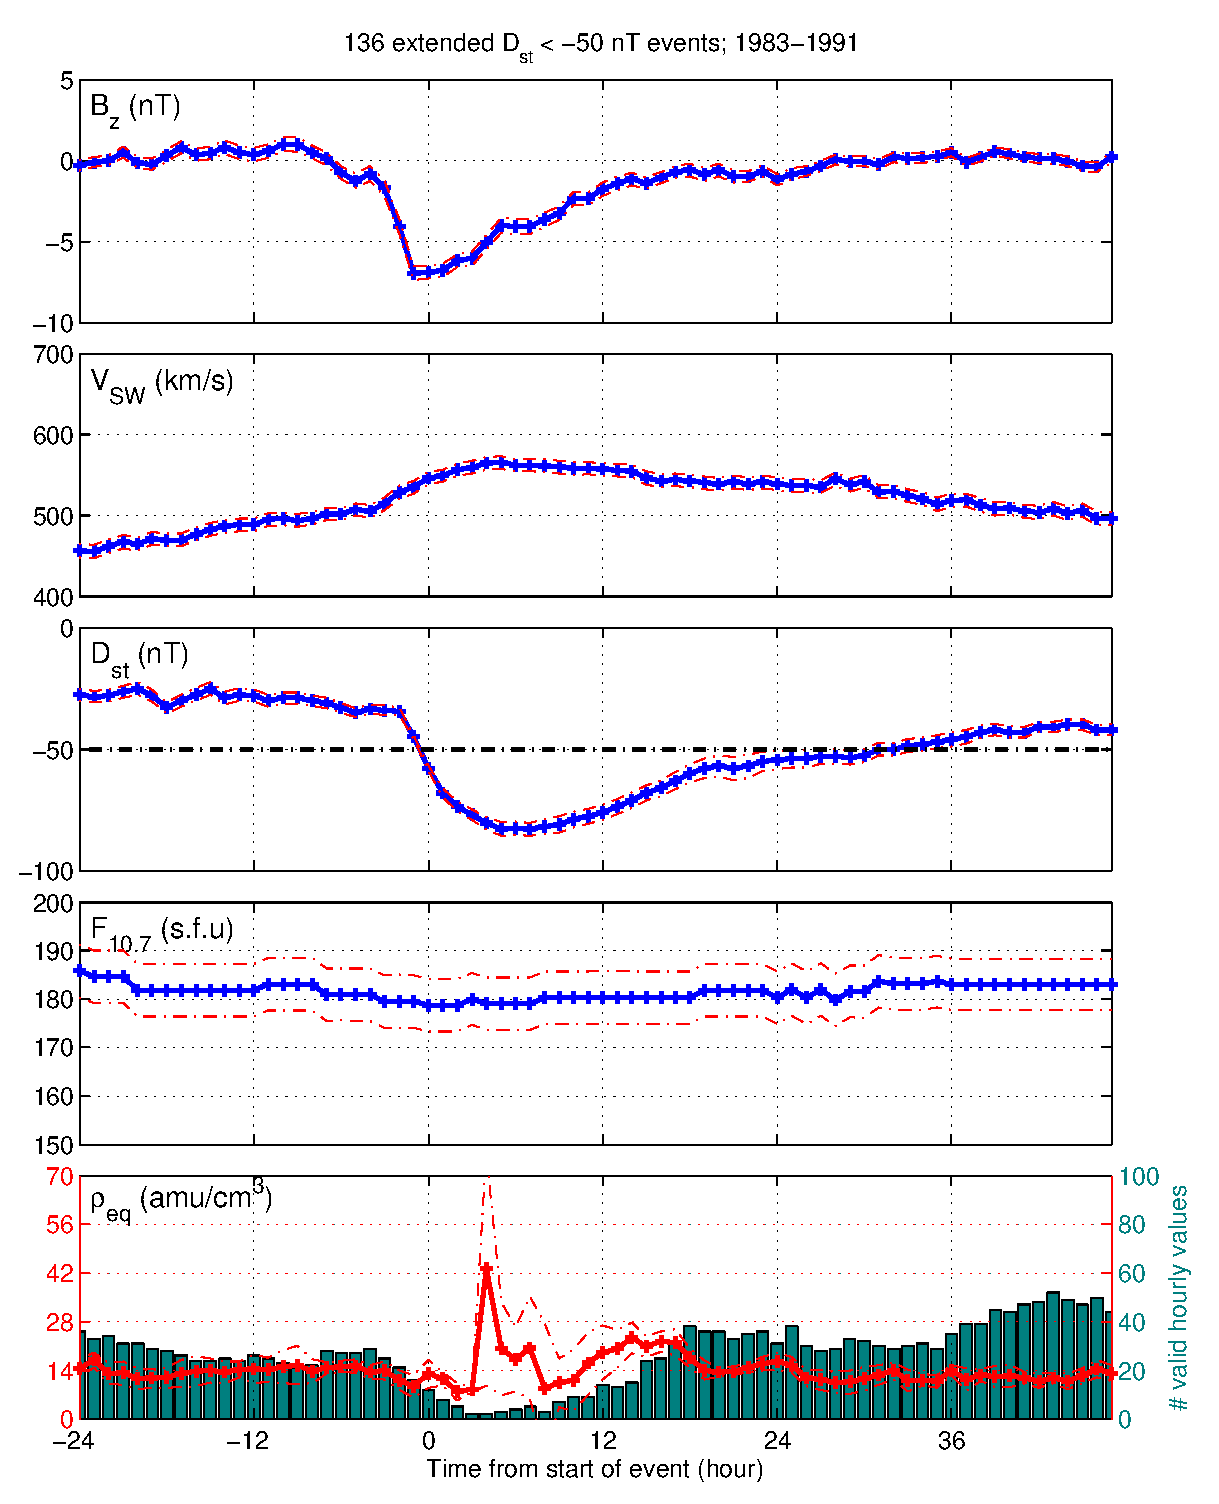
\includegraphics[scale=0.40]{figures/stormavs-dd12-GOES6.eps}
\caption{$D_{st}$ events from GOES 6 using hourly medians. Top: Events in the interval 1983-1991; compare to bottom panel {DailyAveragedDstEvents}. Bottom: Same as Top except for constraint that $D_{st}$ stayed below $-50$~nT for at least 12~hours after crossing below $-50$~nT.}
\label{HourlyAveragedDstEvents}
\end{figure}

\clearpage

\begin{figure}[htp!]
\centering
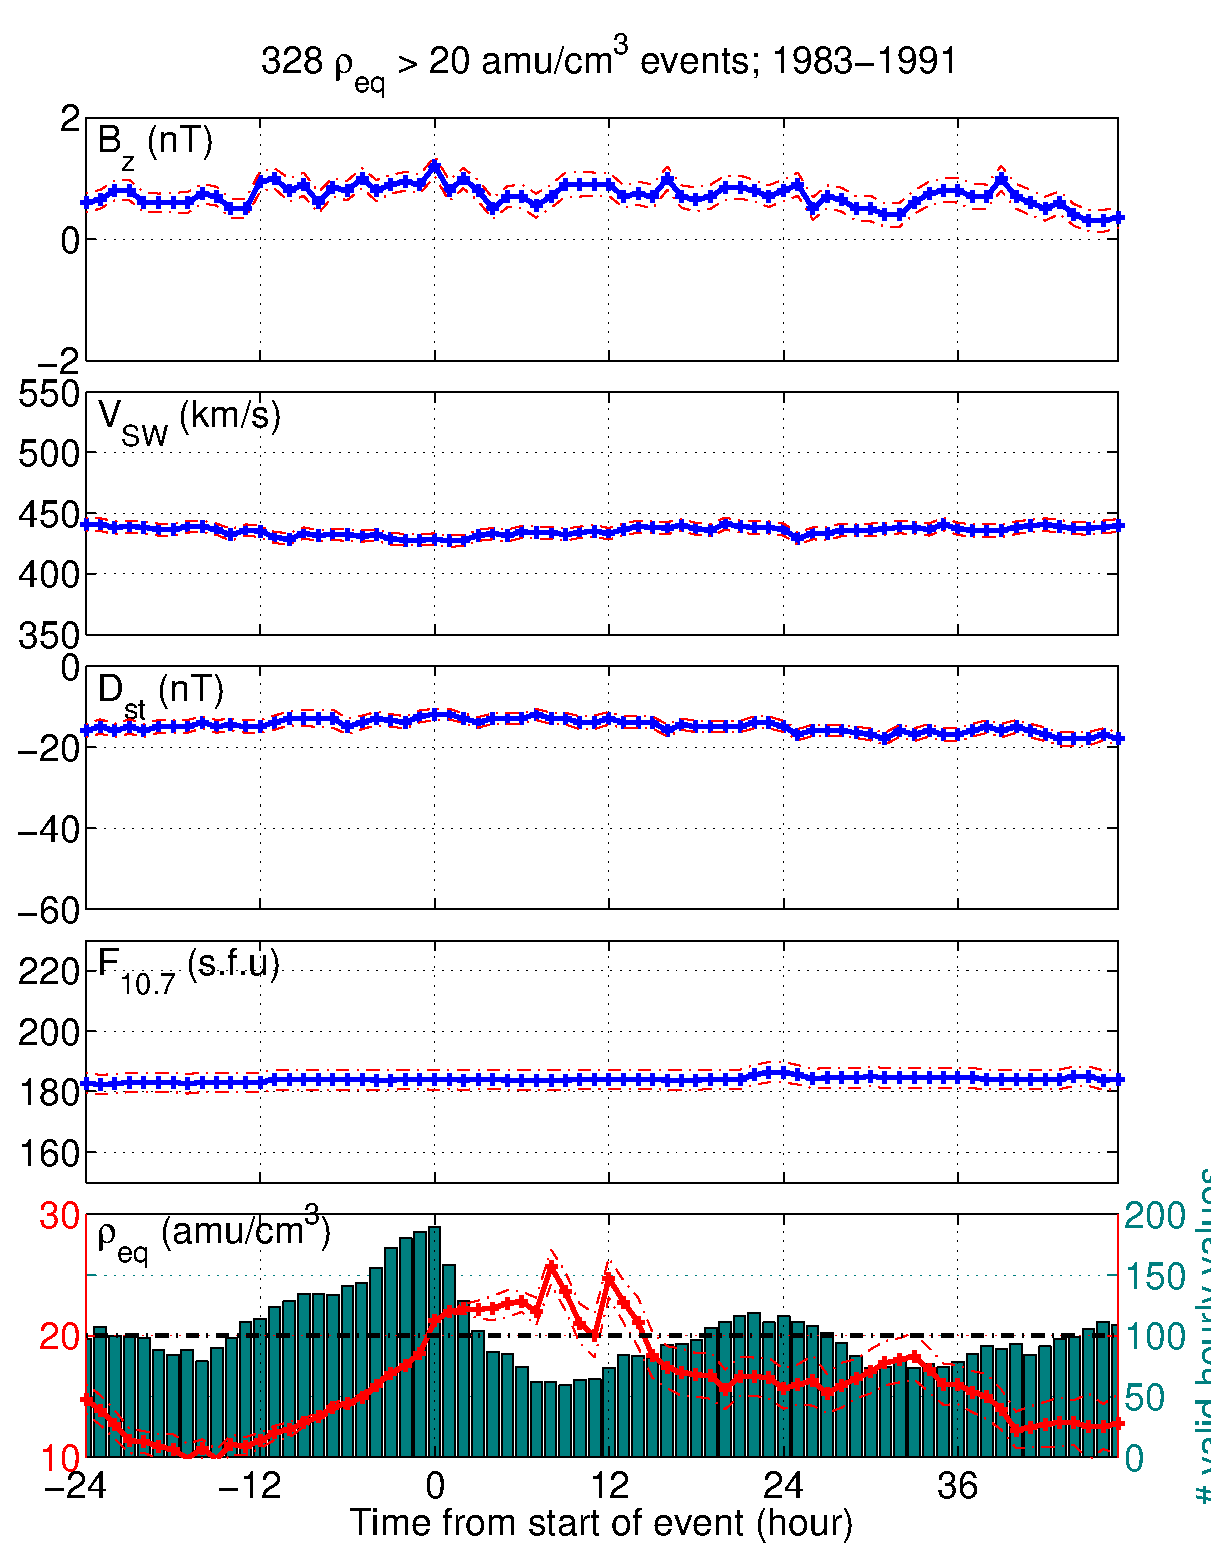
\includegraphics[scale=0.40]{figures/stormavs-mass-gt20-GOES6.eps}
\caption{$\req\ > 20$~ amu/cm$^3$ events from GOES 6 using hourly medians. As described in the text, there is no statistically significant dependence of the \req\  plot on $B_z$ in the time interval of $\pm 2$~hours around the event.}
\label{HourlyAveragedRhoEvents}
\end{figure}

\begin{figure}[tp!]
	\centering
	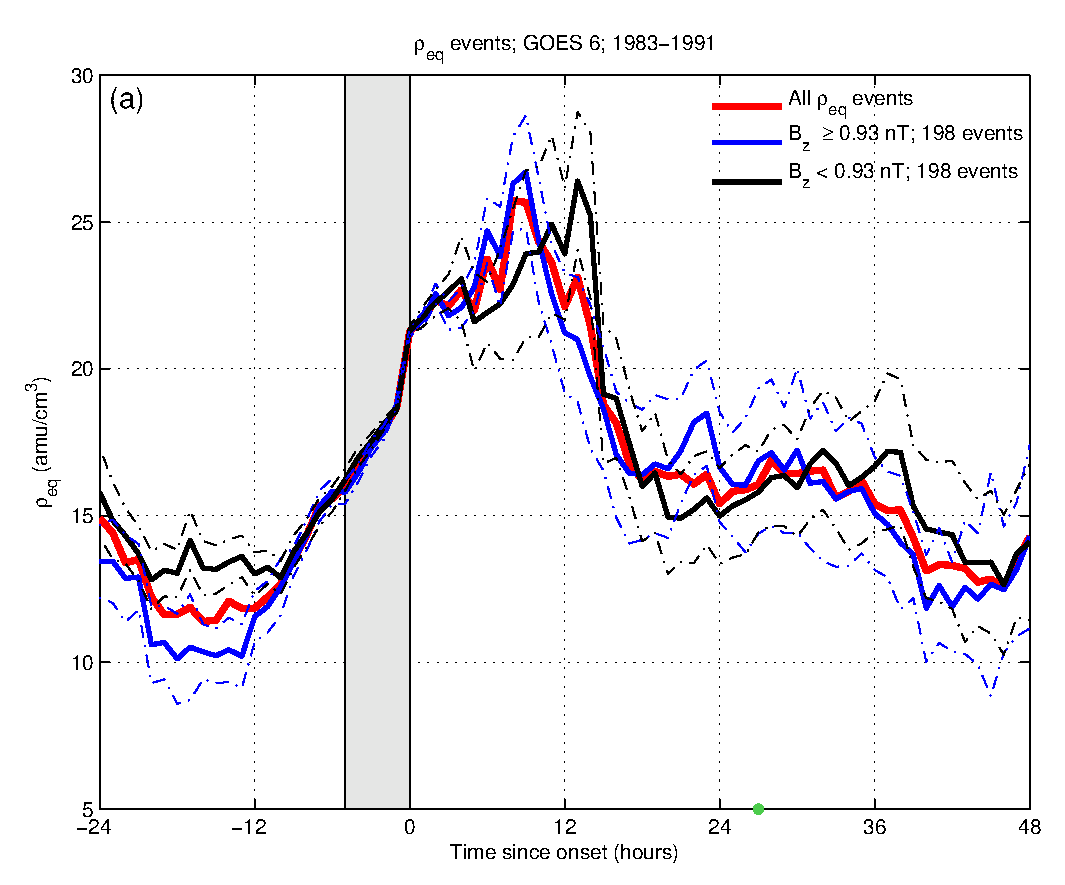
\includegraphics[scale=0.40]{figures/RhoBinnedBz-case24-t020-tf25-GOES6.eps}
	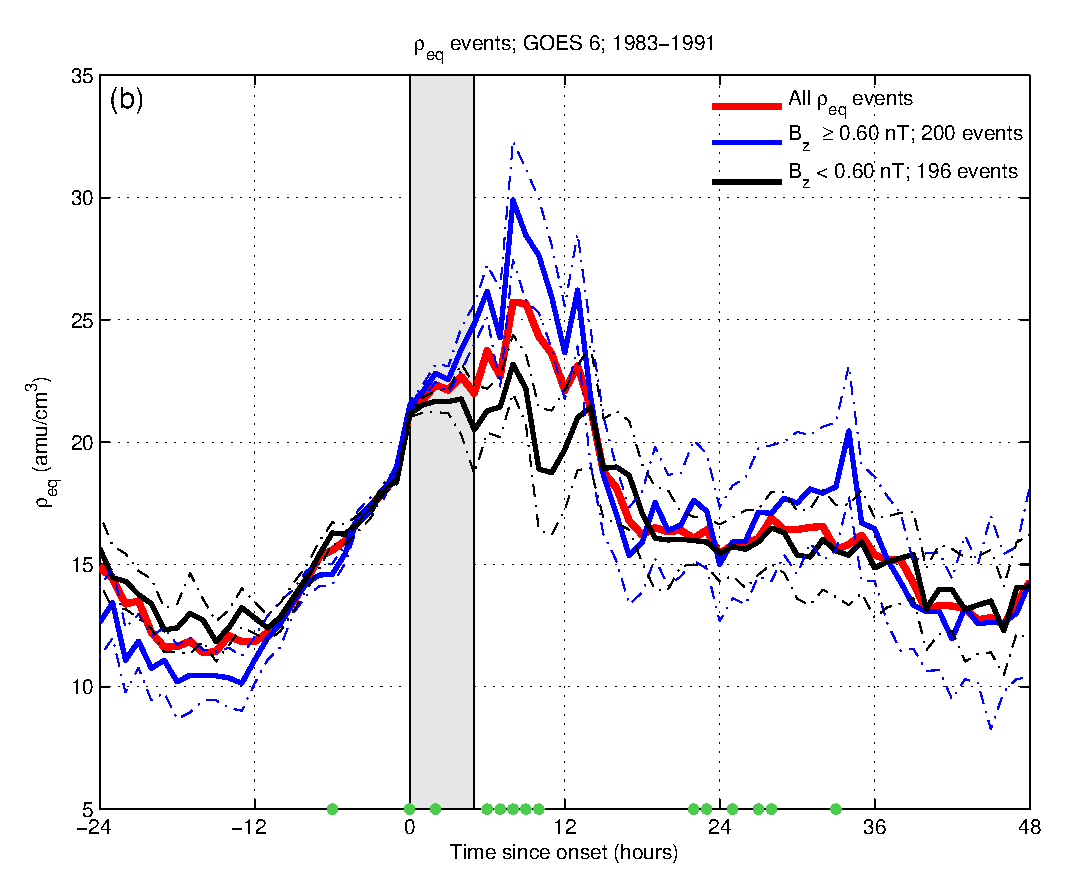
\includegraphics[scale=0.40]{figures/RhoBinnedBz-case24-t025-tf30-GOES6.eps}
	\caption{Binning \req\ events by $B_z$ value (a) at onset and four hours before, and (b) at onset and four hours after.}
	\label{fig:RhoBinned}
\end{figure}


\end{document}
